%\documentclass[10pt]{beamer}
\documentclass[handout, 10pt]{beamer} %handout -> collapse pauses

% MANAGE HANDOUT
%\usepackage{pgfpages} 
% \setbeameroption{show notes}
% \setbeameroption{show notes on second screen=right}

\usepackage{../preamble_slides}
\usepackage{../macros}

\usetheme{metropolis}

%%% Remove nav symbols (and shift any logo down to corner)
\setbeamertemplate{navigation symbols}{\vspace{-2ex}}

\title{Random vectors in high dimensions}
\author{Dimitri Meunier}
\institute{IIT}

\begin{document}
\maketitle

\begin{frame}
  \frametitle{Plan}

  \begin{enumerate}
  \item Random vectors
    \pause
  \item Characteristic function
    \pause
  \item Gaussian vectors
    \pause
  \item Sub-Gaussian vectors
    \pause
  \item Uniform probability measure on the sphere
  \end{enumerate}
\end{frame}



  \section{Refresher: random vectors}

  \begin{frame}
    \frametitle{Random Vectors -- moments}

    A real random vector is a measurable function,

    \begin{align*}
      X \colon (\Omega,\cA,\P) &\to  (\Rd,\cB(\Rd))\\
      w &\mapsto (X_1(w), \ldots, X_d(w))
    \end{align*}

    \pause

    \begin{itemize}
    \item $\E[X] = (\E[X_1], \ldots, \E[X_d])^T \in \Rd$
      \pause
      
    \item $\V[X] = \E[(X-\E[X])(X-\E[X])^T] \pause =  \E[XX^T] - \E[X]\E[X]^T \in
      \R^{d\times d}$
      \pause
    %\item $\mathbb{V}[X]_{ii} = \mathbb{V}[X_i], i=1,\ldots,d$
    \item $\V[X]_{ij} = Cov(X_i,X_j), \quad  i,j=1,\ldots,d$        
    \end{itemize}
  \end{frame}

  % \begin{frame}
  %   \frametitle{Random Vectors -- isotropy}

  %   \textbf{Isotropy:}  $\E[XX^T] = I_d$

  %   \pause

  %   Equivalently,   
 
  %   \begin{itemize}
  %   \item $\E[\langle X,\theta \rangle^2] = \|\theta\|_2^2$ for all $\theta \in
  %     \Rd$
  %   \item $\E[\langle X,\theta \rangle^2] = 1$ for all $\theta \in S^{d-1}$
  %   \end{itemize}

  %   \textbf{Proof} If $A$ and $B$ are symmetric, $A=B$ if and only if
  %   $\theta^TA\theta = \theta^TB\theta$ for all $\theta \in \Rd$.
  % \end{frame}

  \section{Gaussian vectors}

  \begin{frame}{Characteristic function}

    \begin{definition}[Characteristic function]
      if $X$ is a real random vector, the characteristic function of $X$ is the function
      $\Phi_{X}: \mathbb{R}^{d} \longrightarrow \mathbb{C}$ defined by
      $$
      \Phi_{X}(\xi)=\E[e^{i\langle \xi,X \rangle}] = \int_{\Rd} e^{i\langle \xi,X \rangle} \P_{X}(d x), \quad \xi \in \mathbb{R}^{d}
      $$

    where $\P_X(A) = \P(X^{-1}(A))$, for all $A \in \cB(\Rd)$. $\Phi_{X}$ is the Fourier transform of the distribution of $X$.
    \end{definition}

    \pause

    \begin{theorem}
      The characteristic function of a real random vector $X$ characterised its
      distribution: $\Phi_X = \Phi_Y \implies \P_X = \P_Y$.
    \end{theorem}

    \pause

    
    \begin{corollary}
      $X=(X_1,\ldots,X_d)$ has independent coordinates if and only if \\
      $\Phi_{X}\left(\xi_{1}, \ldots, \xi_{d}\right)=\prod_{i=1}^{d}
      \Phi_{X_{i}}\left(\xi_{i}\right)$
    \end{corollary}
  \end{frame}

  \begin{frame}{Univariate Gaussian distribution}

    The univariate standard normal (or Gaussian) random variable  $Z \sim
    \cN_1(0,1)$, is the random variable with density function,
    $$f_Z(x)=(2\pi)^{-\frac{1}{2}} e^{-\frac{1}{2}x^{2}}.$$

    \pause

    $X \sim \cN_1(\mu,\sigma^2)$ if $X = \mu + \sigma Z$
    ($\sigma \geq 0$) where  $Z \sim \cN_1(0,1)$.

    $$f_X(x)=(2
    \pi\sigma^2)^{-\frac{1}{2}} e^{-\frac{1}{2\sigma^2}(x-\mu)^{2}} \qquad
    (\sigma > 0) $$

    \pause

      $$
      \boxed{\Phi_{X}(\xi)=\exp \left(i\xi \mu -\frac{\sigma^{2} \xi^{2}}{2}\right), \quad \xi \in \mathbb{R}}
      $$

      \pause

      \textbf{Proof}. It is sufficient to show that $\Phi_{Z}(\xi)=\exp
      \left(-\frac{\xi^{2}}{2}\right)$. For this, use integration by parts to
      show that $\Phi_Z$ satisfies $\Phi_Z'(\xi) = -\xi\Phi_Z(\xi)$, $\Phi_Z(0) =
      1$.
  \end{frame}

  \begin{frame}{Gaussian vectors -- definition}
    \begin{definition}
      Let $X:(\Omega,\cA,\P) \to \Rd$ be a real random vector. $X$ is a \textbf{Gaussian
        vector} if for all $\theta \in \Rd$, $\langle X, \theta \rangle$ has a
      univariate normal distribution.
    \end{definition}

    \pause

    \begin{theorem} $X$ is a Gaussian vector if and only if, there exists a
      vector $\mu \in \mathbb{R}^{d}$ and a positive semi-definite matrix $K \in \R^{d \times d}$ such that,

      \begin{equation}
        \Phi_{X}(\xi)=\exp \left(i \mu \cdot \xi-\frac{1}{2} \xi^t K \xi\right),
        \qquad \xi \in \Rd.
      \end{equation}

      Furthermore, $\mu = \E[X]$ and $K = \mathbb{V}(X)$, we use the notation
      $X \sim \cN_d(\mu,K)$.
    \end{theorem}

    \pause
    \textbf{Proof.}
  \end{frame}

  \begin{frame}{Gaussian vectors -- properties}

    \begin{corollary}
      \begin{itemize}
      \item If $X$ is a Gaussian vector, its coordinates are independant if and only if
        the covariance matrix is diagonal.

        \pause

      \item If $X$ is a vector of independent univariate
        Gaussian variables, $X$ is a Gaussian vector

      %\item  $X \sim \cN_d(0,I_d)$ if and only if its coordinates are i.i.d with
      %  distribution $\cN(0,1)$. $X$ is called a \textbf{standard Gaussian}
      %  vector.
      \end{itemize}
    \end{corollary}

    \pause

    \begin{proposition}
      If $X$ is a Gaussian vector, for all $B \in \R^{r \times d}$ and $b
      \in \R^r$, $Y = BX + b$ is also a Gaussian vector.
    \end{proposition}
  \end{frame}

  \begin{frame}
    \frametitle{Gaussian vectors -- density}

    \begin{corollary}
      Let $X \sim \cN_d(\mu,K)$, then $X =
      K^{1/2}Z + \mu$, where $Z \sim \cN_d(0,I_d)$ and the equality holds in
      distribution. 
    \end{corollary}

    \pause

    \begin{corollary}
      
      If $X \sim \cN_d(\mu,K)$, $X$ admits a density if and only if $K$ is
      invertible and in that case, its density function is,
      $$f(x)=|2 \pi K|^{-\frac{1}{2}} e^{-\frac{1}{2}\|x - \mu\|_{K^{-1}}^{2}}$$
    \end{corollary}
  \end{frame}

  \begin{frame}{Sub-Gaussian vectors -- definition}
    \begin{definition}[Sub-gaussian random vector] A random vector $X$ in
      $\mathbb{R}^{d}$ is called sub-gaussian if the one-dimensional marginals
      $\langle X, \theta \rangle$ are sub-gaussian random variables for all $\theta \in \mathbb{R}^{d} .$ The sub-gaussian norm of $X$ is defined as
      $$
      \|X\|_{\psi_{2}}=\sup _{\theta \in S^{d-1}}\|\langle X, \theta\rangle\|_{\psi_{2}}
      $$

    \end{definition}

    \pause

    \textbf{Examples.}
    
    \begin{itemize}
    \item Gaussian vectors
    \item Random vectors with \emph{independent} sub-gaussian coordinates
    \item Uniform distribution on the sphere (next section)
    \end{itemize}
  \end{frame}

  \begin{frame}{Spherical distribution}

    \begin{columns}
      \begin{column}{0.75\textwidth}

        \begin{definition}
          If $A \in \mathcal{B}\left(S^{d-1}\right)$, we define the \emph{wedge}
          $\Gamma(A)$ as the Borel set
          of $\mathbb{R}^{d}$ defined by
          $$
          \Gamma(A)=\{r x ; r \in[0,1] \text { and } x \in A\}
          $$
          \pause
          The \textbf{spherical measure} on the sphere is defined by,
          $$
          \omega_{d}(A)=\lambda_{d}(\Gamma(A))
          $$
        \end{definition}
      \end{column}
      \pause
      \begin{column}{0.25\textwidth}  %%<--- here
        \begin{center}
          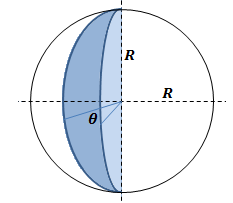
\includegraphics[width=1\textwidth]{wedge.png}
        \end{center}
      \end{column}
    \end{columns}

    \pause

    It can be shown that $\omega_d(S^{d-1}) = \lambda_d(B^d)  = \frac{\pi^{d /
        2}}{\Gamma\left(\frac{d}{2} + 1\right)} $.
    \pause

    \begin{equation*}
      \sigma_{d}(A):= \omega_d(S^{d-1})^{-1} \omega_d(A)
    \end{equation*}

    is the \textbf{uniform probability distribution on the sphere}.

  \end{frame}

  \begin{frame}{Polar change of variables}
    \begin{theorem}
      \begin{itemize}
      \item $\sigma_{d}$ is the unique probability measure on the sphere
        $S^{d-1}$ invariant to the action of vectorial isometries.

        \pause

      \item For any measurable function $f: \Rd \to \R$ positive or integrable,

        \begin{equation*}
          \begin{aligned}
            \int_{\R^{d}} f(x) d x &=\int_{S^{d-1}}\left(\int_{0}^{\infty} f(r \gamma) dr^{d-1} d r\right) d \textcolor{blue}{\omega_d}(\gamma) \\ \pause
            &= \textcolor{blue}{\omega_d(S^{d-1})} \int_{S^{d-1}}\left(\int_{0}^{\infty} f(r \gamma) dr^{d-1} d r\right) d \textcolor{blue}{\sigma_d}(\gamma)
          \end{aligned}
        \end{equation*}


      \end{itemize}

    \end{theorem}

  \end{frame}

  \begin{frame}{Link to the Gaussian distribution}
    \begin{proposition}[Exercise 3.3.7] Let us write $X \sim N_d\left(0, I_{d}\right)$ in
      polar  form as
      $$
      X=R \theta
      $$
      where $R=\|X\|_{2}$ is the length and $\theta=X /\|X\|_{2}$ is the direction
      of $X$. Prove the following:

      \pause

      \begin{enumerate}
      \item the length $R$ and direction $\theta$ are independent random
        variables
        \pause
      \item the direction $\theta$ is uniformly distributed on the unit sphere
        $S^{d-1}$
      \end{enumerate}
    \end{proposition}

  \end{frame}

  % \begin{frame}{Gaussian concentration}
  %   \begin{itemize}
  %   \item recall concentration of the norm
  %   \item fine tune the interpretation for Gaussian (+ images)
  %   \item Isotropy / Sub-Gaussianity of the uniform sphere r.v.
  %   \item Examples of sub-gaussianity
  %   \end{itemize}
  % \end{frame}
\end{document}
